\chapter{wafamole++}
\label{chp:capitulo4}

Tendo em consideração o embasamento teórico estabelecido e a oportunidade de contribuir para um projeto \textit{open source} na área de interesse deste trabalho que tivesse uma boa abrangência e impacto, foi concebido o \textbf{wafamole++}, uma versão estendida do WAF-A-MoLE anteriormente descrito no capítulo de Revisão de Literatura. Foram seguidas diretrizes e recomendações de contribuição estabelecidas pelos autores, e alguns módulos adicionais contendo funcionalidades não disponibilizadas pelos mesmos referentes ao treinamento de novos classificadores, geração de novos modelos, e tratamento de datasets foram disponibilizados com este trabalho.

A elaboração do mesmo permitiu um entendimento mais profundo da ferramenta original, recebendo apoio dos autores originais e atualmente conta com uma série de operadores de mutação novos e sobretudo modelos de classificadores novos implementados para um Web Application Firewall de código aberto encontrado na plataforma de colaboração Github.

Acredita-se que essa colaboração ocasionou em uma ferramenta mais abrangente, com uma menor barreira de entrada para futuros colaboradores e mais flexível para avaliação de Web Application Firewalls baseados em Aprendizado de Máquina no geral. Assim espera-se que mais contribuições possam ser geridas no futuro, estabelecendo-se como um projeto complementar ao WAF-A-MoLE original.


\section{Arquitetura}

O cerne do projeto encontra-se nos seguintes módulos:
\begin{alineas}
\item \verb+Main+ - Responsável pela lógica da linha de comando, com todos os decorators da biblioteca \verb+Click+ que facilitam o desenvolvimento de utilidades de terminal. É feito o recebimento e passagem de parâmetros para a pipeline do programa aqui, além de ser instanciada a classe principal \verb+wafamole+ e o módulo \verb+EvasionEngine+ com o modelo selecionado pelo usuário.
\item \verb+models+ - Em models estão localizados os modelos de exemplo para experimentação de desenvolvedores novos, modelos padrões do WAF-A-MoLE e sobretudo modelos novos (também customizáveis) introduzidos no wafamole++, localizados na pasta \verb+/models/svc+. Modelos novos de classificadores de Web Application Firewalls a serem testados são tipicamente arquivos .dump das classes de tais classificadores, gerados através biblioteca \verb+joblib+ após o treinamento (no caso do scikit-learn, da função \verb+.fit()+). Alternativamente, essa biblioteca permite também a geração de um arquivo .dump de uma pipeline caso o treinamento exija mais de uma etapa, como uma Tokenização para possibilitar o treinamento de um dado classificador.
\item \verb+EvasionEngine+ - Essa classe contém o loop principal que requisita as mutações responsáveis pela transformação do payload fornecido pelo usuário em um payload considerado inócuo para o WAF avaliado. As requisições são feitas ao módulo \verb+Fuzzer+.
\item \verb+Fuzzer+ - Nesse módulo ficam armazenados os operadores de mutação que transformam o payload a cada rodada de mutação efetuada, e cada mutação ocorre dentro do mesmo. Um operador de mutação aleatório dentre estes é escolhido a cada iteração da pipeline principal.
\end{alineas}

Esses módulos, no entanto, não podem ser trivialmente estendidos sem alguns componentes auxiliares criados para o wafamole++, que são:
\begin{alineas}
\item \verb+datasets+ - TO-DO
\begin{alineas}
\item \verb+mole+ - TO-DO
\item \verb+sqli_cleaner+ - TO-DO
\end{alineas}
\item \verb+MLBasedWafClassifier+ - TO-DO
\item \verb+MLClassifierWafamole+ - TO-DO
\end{alineas}

\begin{figure}[H]
    \centering
    \caption{Arquitetura do wafamole++}
    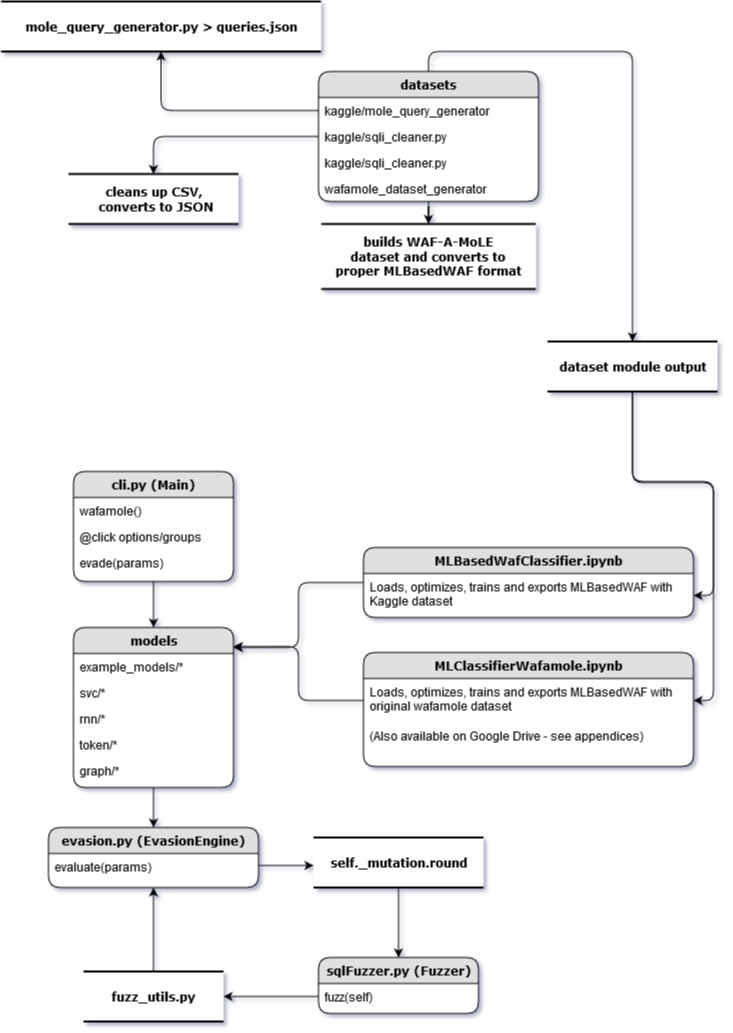
\includegraphics[width=16cm]{figuras/wafamole++_architecture.png} 
    \legend{Fonte: Elaboração Própria (2022)}
    \label{fig:internet} 
\end{figure}

\section{WAFs avaliados}

\subsection{WAF-Brain}

\textbf{Autores}: Sergio D Fdez, cr0hn, Enrique Garcia. Disponível no Github \href{https://github.com/BBVA}{BBVA}

O WAF-Brain foi um dos primeiros firewalls a serem testados pela equipe do WAF-A-MoLE, e subsequentemente é o primeiro modelo de exemplo disponibilizado para testes na documentação do mesmo. Dessa maneira, foi extensivamente testado com os novos operadores de mutação, sendo de grande ajuda para diagnosticar os incluídos no wafamole++.

\begin{figure}[ht]
    \centering
    \caption{Dependências e logomarca do WAF-Brain}
    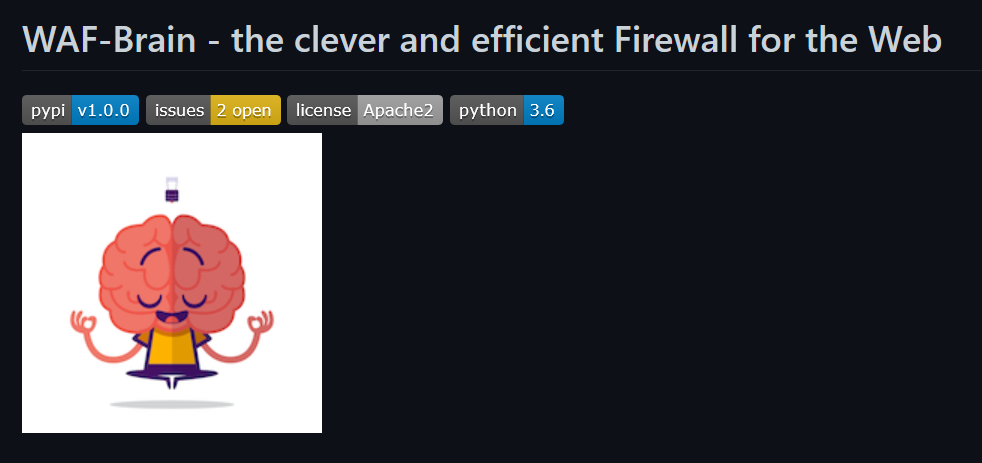
\includegraphics[width=12.5cm]{figuras/WAFBrain.png} 
    \legend{Fonte: \href{https://github.com/BBVA}{Github} (2019, p. TO-DO)}
    \label{fig:internet} 
\end{figure}

Seu funcionamento se dá, como anteriormente mencionado, através da estratégia de Deep Learning com Redes Neurais, pela qual são analisados cada campo de um determinado pedido HTTP sob a ótica de um classificador treinado desta maneira, determinando se esse campo é malicioso ou não.

Na adaptação WAF-A-MoLE, esse poder de predição é aproveitado exclusivamente na forma de probabilidade - tendo a probabilidade de ser uma SQL-Injection acima de um determinado limite, temos um caso malicioso. Isso requer que o classificador treinado no modelo não apenas mostre a previsão, mas também a precisa probabilidade com a qual chegou à mesma.

Por mais que se trate de um algoritmo sofisticado por natureza, surpreendentemente o WAF-Brain fora implementado pelos seus autores originais de uma maneira simplória o suficiente para ser um dos WAFs mais vulneráveis às estratégias de fuzzing do WAF-A-MoLE. Vários operadores de mutação isolados conseguem resultados frutíferos em pouco tempo, como será visto na seção de testes adiante.

\section{Operadores de Mutação}

\section{Modelos}
Todos os modelos implementados tiveram como base o firewall ML-Based-WAF, disponível por vladan-stojnic no \href{https://github.com/vladan-stojnic/ML-based-WAF}{Github} que fora o WAF open source mais promissor e mais plausível de adaptar. Sua performance também era factível no contexto de recursos disponíveis para a conclusão deste projeto final.

\begin{figure}[ht]
    \centering
    \caption{Repositório ML-Based-WAF}
    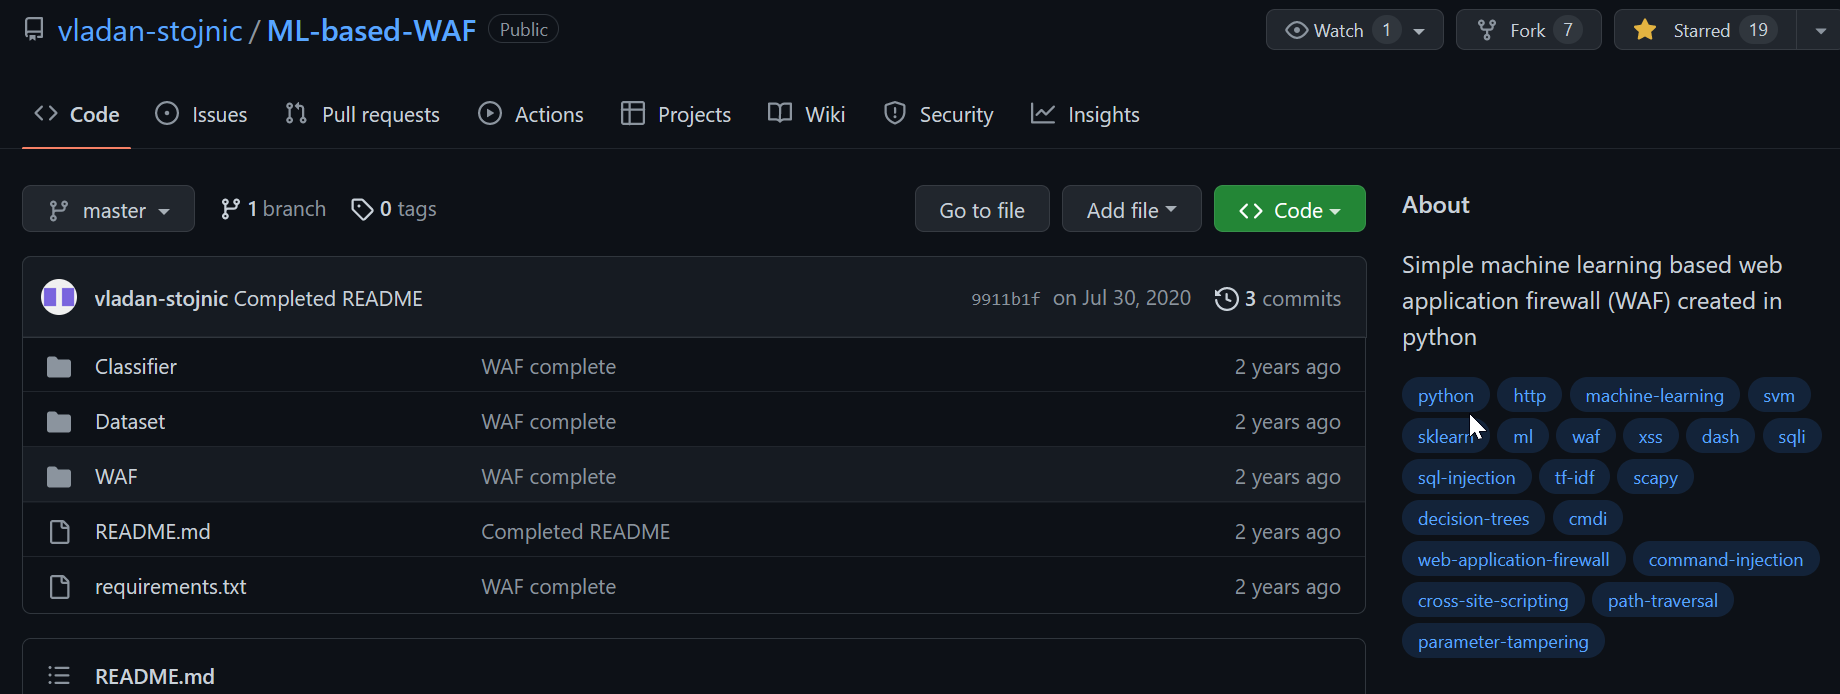
\includegraphics[width=16cm]{figuras/MLBasedWAF.png} 
    \legend{Fonte: \href{https://github.com/vladan-stojnic/ML-based-WAF}{Github} (2020, p. TO-DO)}
    \label{fig:internet} 
\end{figure}

Embora seja um WAF orientado ao tráfego real ou simulado de uma rede de fato, avaliando parâmetros HTTP em tempo real no seu componente sniffer.py tanto por SQL-Injections como por outras formas de ataque (XSS, cmdi e outras), ainda foi possível restringir seu funcionamento para adaptá-lo ao wafamole++. 

Para tal, foi necessário prever uma estratégia própria de treinamento para o classificador, além de um conjunto de dados especial para o mesmo. É cabível mencionar, no entanto, que isso introduziu uma série de dificuldades uma vez que sua documentação era consideravelmente modesta, e o banco novo a ser usado deveria seguir o padrão de formatação seguido pelo WAF.

Dentre as opções de datasets disponíveis com SQL Injections, foi escolhido inicialmente a versão SQLiV3.json da coleção do Kaggle que será amostrada a seguir.
Além disso, para corrigir uma variedade de erros de formatação, polir algumas queries incorretas (e de difícil proveito), e finalmente adaptar para o padrão .json utilizado pelo WAF, a seguinte função auxiliar foi codificada:

\begin{figure}[ht]
    \centering
    \caption{Detalhes Dataset SQL Injection Kaggle.}
    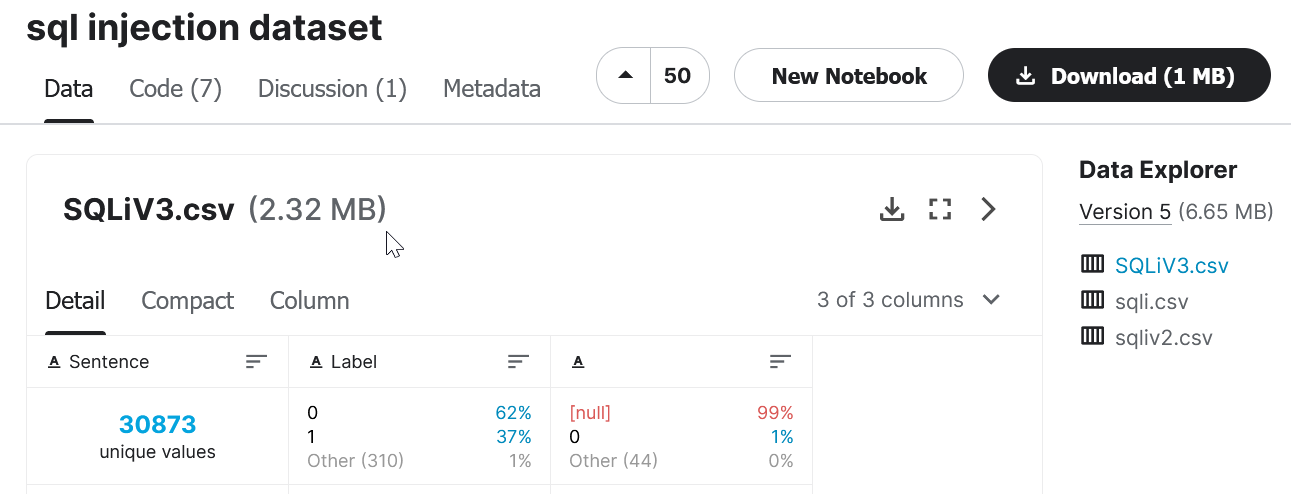
\includegraphics[width=16cm]{figuras/sqlInjectionDataset.png} 
    \legend{Fonte: \href{https://www.kaggle.com/datasets/syedsaqlainhussain/sql-injection-dataset}{Kaggle} (2021, p. TO-DO)}
    \label{fig:internet} 
\end{figure}

\label{sec:codigos}
\includecode[C]{Para tratamento de dados brutos} {alg:codigo3}{codigos/sqli_cleaner.py}

\subsection{Support Vector Machine}
Este foi o primeiro modelo implementado no wafamole++, antes do recebimento do dataset original da equipe original. 





